% ------------------------------------------------------------------------------
% TYPO3 v9 LTS - What's New (English Version)
%
% @author	Michael Schams <schams.net>
% @license	Creative Commons BY-NC-SA 3.0
% @link		https://typo3.org/help/documentation/whats-new/
% @language	English
% ------------------------------------------------------------------------------

\section{Privacy and Security}
\begin{frame}[fragile]
	\frametitle{Privacy and Security}

	\begin{center}\huge{\color{typo3darkgrey}\textbf{Privacy and Security}}\end{center}
	\begin{center}\large{\textit{General Data Protection Regulation (GDPR) and more...}}\end{center}

\end{frame}

% ------------------------------------------------------------------------------
% General Data Protection Regulation

\begin{frame}[fragile]
	\frametitle{Privacy and Security}
	\framesubtitle{Anonymize IP Addresses}

	\begin{itemize}
		\item Scheduler task can be activated to anonymize IP addresses in
			several database tables after a certain period of time
		\item For example table \texttt{sys\_log}, after 30 days:
			\begin{figure}
				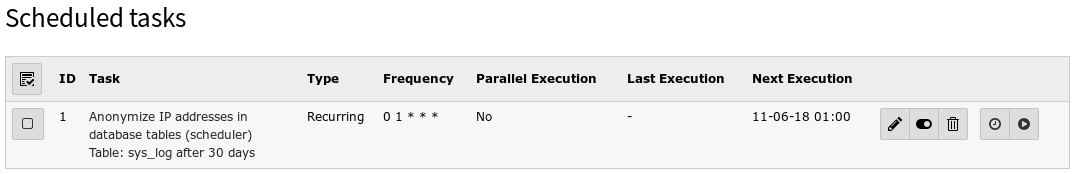
\includegraphics[width=1\linewidth]{PrivacyAndSecurity/IpAnonymizationSchedulerTask.png}
			\end{figure}
		\item You can find more information on GDPR on the \href{https://typo3.com/blog/tag/gdpr/}{TYPO3 GmbH Blog}
	\end{itemize}

\end{frame}

% ------------------------------------------------------------------------------
% FE/BE User Accounts and Passwords
% #85026 - salted passwords changes

\begin{frame}[fragile]
	\frametitle{Privacy and Security}
	\framesubtitle{FE/BE User Accounts and Passwords}

	% decrease font size for code listing
	\lstset{basicstyle=\tiny\ttfamily}

	\begin{itemize}
		\item Plain text passwords are not longer possible for BE/FE users at all
		\item Inactive FE/BE user records can now be removed from the database by
			adding scheduler task "Table garbage collection task" and enabling
			"Clean all available tables"\newline
			\smaller
				(data that does not exist, cannot be compromised in case of a
				security breach)
			\normalsize

\begin{lstlisting}
<?php
$tableGarbageCollectionTask = \TYPO3\CMS\Scheduler\Task\TableGarbageCollectionTask::class;
$GLOBALS['TYPO3_CONF_VARS']['SC_OPTIONS']['scheduler']['tasks'][$tableGarbageCollectionTask]
  ['options']['tables'] = [
  'be_users' => [
    'dateField' => 'lastlogin',
    'expirePeriod' => 30
  ]
];
\end{lstlisting}

		\item See \href{https://docs.typo3.org/typo3cms/extensions/scheduler/Installation/BaseTasks/Index.html}{documentation}
			for further details
	\end{itemize}

\end{frame}

% ------------------------------------------------------------------------------
% #84843 - Use no-cookie domain for youtube by default

\begin{frame}[fragile]
	\frametitle{Privacy and Security}
	\framesubtitle{No-cookie Domain for YouTube Videos}

	% decrease font size for code listing
	\lstset{basicstyle=\tiny\ttfamily}

	\begin{itemize}
		\item YouTube videos are rendered by accessing the no-cookie domain
			\url{https://www.youtube-nocookie.com} by default
		\item The regular domain \texttt{www.youtube.com} can be forced by
			the following TypoScript configuration, if required:

\begin{lstlisting}
lib.contentElement {
  settings {
    media {
      additionalConfig {
        no-cookie = 0
      }
    }
  }
}
\end{lstlisting}

	\end{itemize}

\end{frame}

% ------------------------------------------------------------------------------
% Password Hashing API

\begin{frame}[fragile]
	\frametitle{Privacy and Security}
	\framesubtitle{Password Hashing API}

	\begin{itemize}
		\item TYPO3 now uses the
			\href{https://secure.php.net/manual/en/ref.password.php}{PHP Password Hashing API},
			which features algorithms, such as
			\href{https://en.wikipedia.org/wiki/Argon2}{Argon2i}
			and
			\href{https://en.wikipedia.org/wiki/PBKDF2}{PBKDF2}
	\end{itemize}

	\begin{figure}
		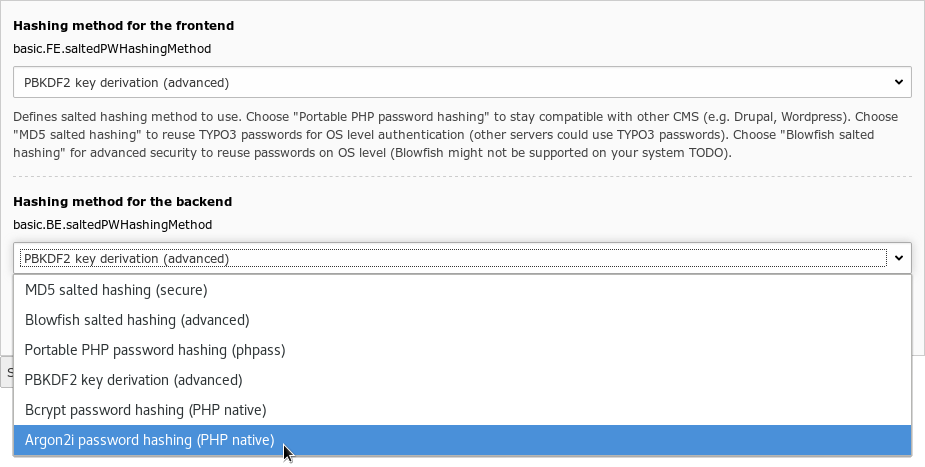
\includegraphics[width=0.7\linewidth]{PrivacyAndSecurity/PasswordHashingAlgorithms.png}
	\end{figure}

\end{frame}

% ------------------------------------------------------------------------------
% Password Hashing API

\begin{frame}[fragile]
	\frametitle{Privacy and Security}
	\framesubtitle{Password Hashing API}

	\begin{itemize}
		\item Integrators can choose between several password hashing methods
			for FE and BE user passwords
		\item Given that MD5 is deemed highly insecure to protect passwords
			today, the support of MD5 hashes has been dropped
		\item If necessary, password hashes are automatically updated when users
			log in
	\end{itemize}

\end{frame}

% ------------------------------------------------------------------------------
